\chapter{Large Language Models}\label{ch:techOverview}

Creating machines with human-like language understanding has been a subject of research since the 1950s.
\gls{natural-language}s are highly complex and pose a difficult challenge to computers.
% ambiguous: ~\autocite{quadarLM2020}
\gls{lm} is an approach to make machines read, write and communicate like humans~\autocite{zhao2023survey}.

The main idea of \gls{lm} is to estimate probability distributions over units of texts, e.g.\ words~\autocite{de2015survey}.
Assuming that the occurrence of a word depends on previous words, i.e.\ the context, the probability of that word being next in a sentence can be modeled with a conditional probability~\autocite{jozefowicz2016exploring}.
\[
    P(w_n | w_1, \dots , w_{n-1})
\]
% TODO: quelle finden vielleicht
The ability to estimate the probability distributions over words makes it possible to predict the next word for a given sequence.
In this way, language models can be applied in many \gls{nlp} tasks like speech recognition, machine translation and text summarization~\autocite{jozefowicz2016exploring}.
By simply predicting the next word, language models can hold human-like conversations, which makes it appear as if they understand natural language.
% How would translation look like?
% TODO: Other approaches like BERT Masked language Modeling
%Other approaches to \gls{lm} mask parts of sentences and use all surrounding language units to predict the missing

There are different techniques to model these probabilities of word sequences.
In the 1990s, \glspl{slm} found widespread use.
The models often assume that the distribution of a word only depends on a fixed length of previous words.
\enquote{$n$-grams models} are \glspl{slm} that use the previous $n$ words to calculate the probability distribution of the next word.
Based on a training corpus, tables of conditional probabilities are created.
The probabilities are approximated by counting occurrences of $n$-grams.
If the previous word is \enquote{thank}, the probability that the next word is \enquote{you} could be estimated as follows~\autocite{quadarLM2020}
\[
    P(\text{you} | \text{thank}) = \frac{P(\text{thank you})}{P(\text{thank})} \approx \frac{count(\text{thank you})}{count(\text{thank})}
\]
In recent years, research has been focused on the more flexible \glspl{nlm}~\autocite{quadarLM2020}.
This approach uses \glspl{dnn} to estimate the needed probability distributions.
\glspl{nlm} are much better at taking long-range depencies in text into account than \glspl{slm}~\autocite{Hadi_2023}.
\glspl{dnn} excel at extracting complex features from text and finding meaningful representations for words.
These representations (often called embeddings) lie in a vector space of real vectors where similar words are close to each other in a mathematical sense~\autocite{quadarLM2020}.
In \glspl{nlm} the prediction function is usually built on top of these embeddings.
The intermediate step of learning effective features and representing them in embeddings has the benefit that those embeddings can be reused for other tasks.
The early 2010s saw the rise of \glspl{dnn} that were specifically designed to create powerful word embeddings~\autocite{zhao2023survey}.
These embeddings were static, meaning the network would assign each word exactly one embedding, disregarding polysemy of words~\autocite{Liu_2020}.
Embeddings of popular solutions like \enquote{word2vec} proved to be very useful in various \gls{nlp}-Tasks.

Following research focused on incorporating context into word embeddings, i.e.\ assigning a different vector representation to a word depending on the surrounding words.
ELMo, BERT and GPT are well-known models that managed to do so.
These context-aware language models are trained on large unlabeled corpora of text data.
During training, the models learn to solve pre-training tasks that are specifically designed for the language model to gain essential language understanding.
They are often put into their own class of language models, the so-called \glspl{plm}.
\glspl{plm} set new standards in solutions of many \gls{nlp}-tasks.
They learn general-purpose features that can be effectively used by fine-tuning the models on downstream tasks, e.g.\ machine translation, text summarization or \gls{ats}.
The process of using a \gls{plm} as a base model to fine-tune it for a specific task has become a commonly used pattern in \gls{lm}~\autocite{zhao2023survey}.

The availability of huge datasets and powerful computing devices led to another evolution in \gls{lm}.
\glspl{llm} are \glspl{plm} that are scaled in model size.
They are usually based on the popular transformer architecture~\autocite{Hadi_2023} and consist of billions of parameters.
Research found that using larger models with more extensive pre-training on larger datasets greatly improves performance~\autocite{Raiaan2024ARO}.
\glspl{llm} even show unexpected abilities (called emergent abilities) that could not be observed in smaller models, e.g.\ reasoning and solving complex tasks without fine-tuning~\autocite{zhao2023survey}.
They are capable of \enquote{in-context learning} meaning they can perform tasks given only instructions and a few examples without the need of updating model parameters~\autocite{bhatia2023tart}.
ChatGPT is an example of a popular \gls{LLM} with amazing conversation and task solving abilities~\autocite{zhao2023survey}.

While \glspl{llm} produce impressive results with \enquote{in-context learning} they are usually still outperformed by fine-tuned language models in specific tasks~\autocite{bhatia2023tart}.
In the context of German \gls{ats} this is supported by the results of~\textcite{deilen2023using} who find that ChatGPT can only create very rudimentary simplifications.

The course of action for this thesis is to use pre-trained base models to fine-tune them on the task of \gls{ats}.
Due to hardware limitations, only \glspl{plm} with up to 13 billion parameters come into question.
In the following sections the underlying workings of \glspl{nlm}, \glspl{plm} and \glspl{llm} will be explained.

% TODO
\begin{figure}
    \centering
    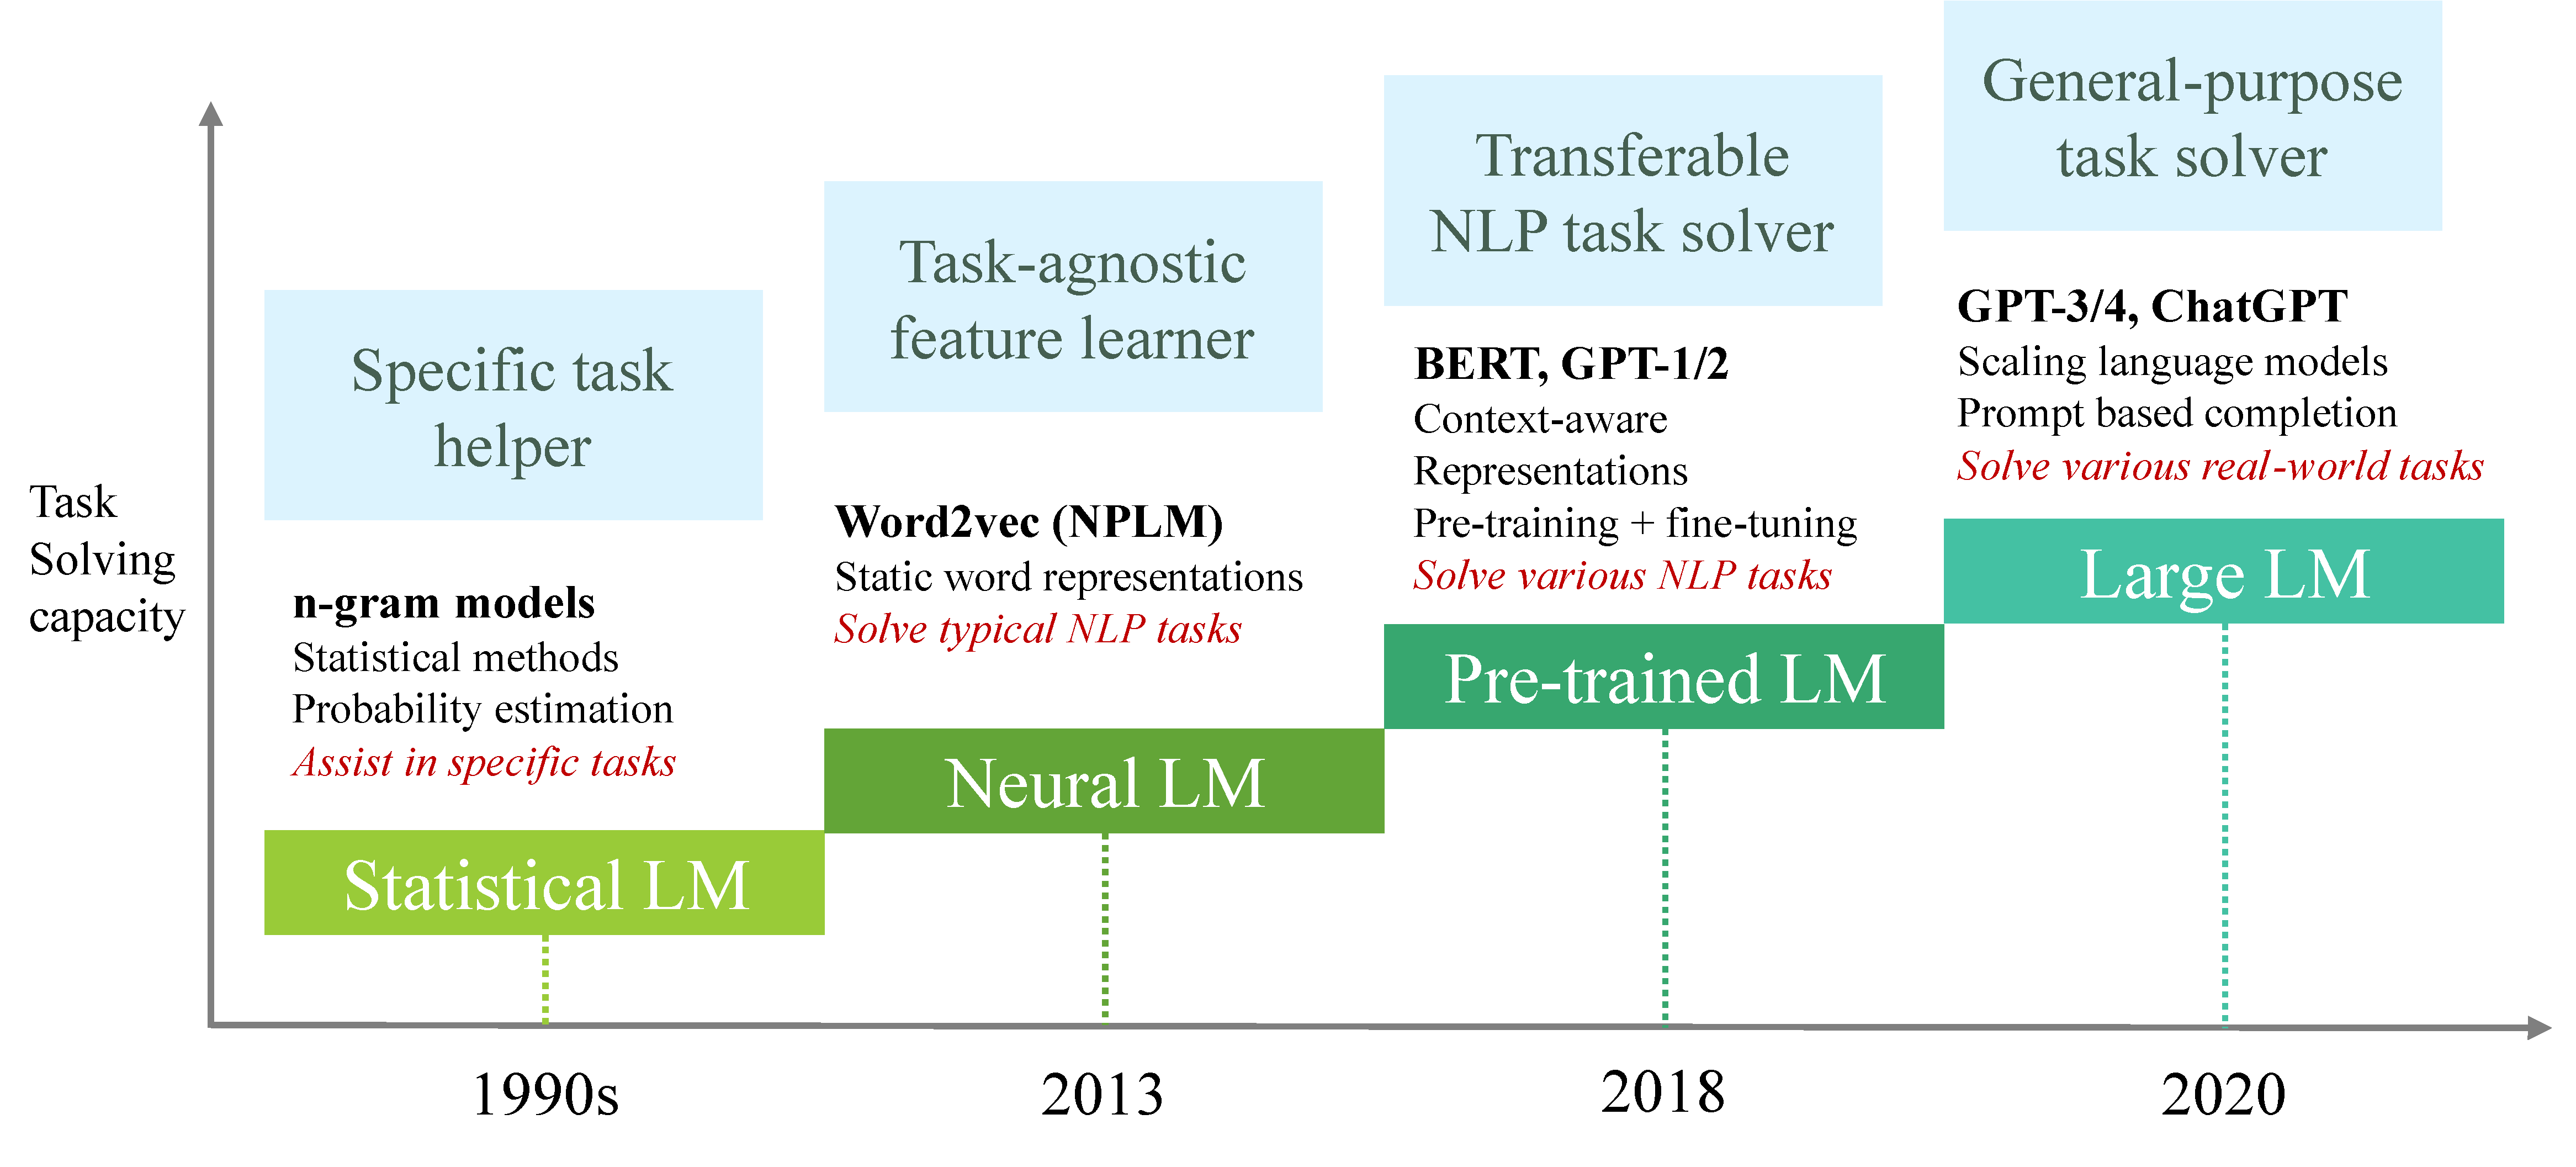
\includegraphics[width=\linewidth]{images/languagemodels}
    \caption[TODO.]{TODO~\autocite{zhao2023survey}}
    \label{fig:language-models}
\end{figure}

%With the introduction of the transformer architecture in 2017~\autocite{vaswani2023attention}
%task-agnostic representations -> less human feature engineering~\autocite{zhao2023survey}

%from~\autocite{zhao2023survey}:
%language modeling to task solving

%from ~\autocite{Raiaan2024ARO}:
%pre-training on large corpora from the web -> learning complicated patterns and language subtleties
%fine-tuning on downstream tasks gives state-of-the-art performance
%"comprehend, produce, forecast human language"

%From ~\autocite{Hadi_2023}:
%during pre-training: models see diverse texts and learn grammar, facts, reasoning

\clearpage

\section{Deep Learning}\label{sec:deep-learning}
As previously mentioned, \glspl{dnn} are the underlying technology for modern language models.
\glspl{dnn} belong to the field \enquote{Deep Learning} which is a specific type of \gls{ml}.
The term \acrlong{ml} describes different computational methods that can learn to perform different tasks from experiencing data~\autocite{Goodfellow-et-al-2016}.

A typical application for \gls{ml} is to learn a task that can be represented by a mapping:
\[
    f: \mathcal{X} \rightarrow \mathcal{Y}
\]
The \textit{input space} $\mathcal{X}$ is the set of all possible \textit{examples}.
Each example is mapped to a \textit{label} or \textit{target value} from the \textit{target space} $\mathcal{Y}$.
Input spaces often consist of real vectors $\boldsymbol{x} \in \mathbb{R}^n$.
The entries $x_i$ of an example vector are called \textit{features}.
Target spaces vary depending on the specific task.
Typical are subsets of natural numbers for \textit{classifications} or real numbers (e.g.\ for \textit{regression}).

For classification tasks, the learned function assigns an integer representing a category to each possible input example.
A common use case for this is the categorization of images.
An automatic image classifier $f:\mathbb{R}^n \rightarrow \{1,\dots,k\}$ receives an image (usually in the form of a real vector) and outputs a numerical value that symbolizes the content of that image e.g.\ a person, an object or an animal.

\gls{ml} offers a broad range of methods to find functions that can model complex behavior.
They incorporate many elements from different fields like linear algebra, probability theory, numerical optimization and information theory~\autocite{Goodfellow-et-al-2016}.
\gls{ml} has been successfully applied to numerous problems from different domains, including text classification, \gls{nlp}, speech processing applications, computer vision and computational biology applications.
\gls{ml}-approaches are usually categorized into the different learning scenarios \textit{supervised learning}, \textit{unsupervised learning} and \textit{semi-supervised learning}.
These scenarios differ in the usage and type of available training data~\autocite{mohri2018foundations}.
Supervised learning is especially relevant for machine translation tasks like \gls{ats}.


\subsection{Supervised Learning}\label{subsec:supervised-learning}
In the setting of supervised learning, available training data consists of pairs of input examples with corresponding target values.
\[
    D = \{(x_1, y_1), \dots, (x_m, y_m)\}
\]
The general aim is to model the relation between the examples $x_i$ and the targets $y_i$.
For that, assumptions about the origin of the data have to be made.
It is commonly assumed that the pairs $(x_i, y_i)$ are sampled from an unknown probability distribution, i.e.\ they are realizations of random variables $Z_i = (X_i, Y_i)$ that take values in $\mathcal{X} \times \mathcal{Y}$.
The random variables $\{(X_1, Y_1), \dots ,(X_m, Y_m)\}$ are independently and identically distributed (i.i.d.) while $X_i$ and $Y_i$ are not necessarily independent~\autocite{gressmann2019probabilistic}.
In the context of \gls{ml} this is often denoted as $(X_i,Y_i) \sim P(X, Y)$ where $P(X, Y)$ signifies the joint probability distribution (e.g.\ \textcite{Goodfellow-et-al-2016}).

In the setting of \enquote{classical} supervised learning, the objective is to learn a deterministic prediction function $f: \mathcal{X} \rightarrow \mathcal{Y}$ that defines a mapping between examples and targets:
\[
    \, (X^*, Y^*) \sim P(X, Y): \quad  Y^* = f(X^*)
\]
To approximate this mapping, a set of potential prediction functions $\mathcal{H}$ is considered.
% TODO example
The learning algorithm consists of choosing the hypothesis $h \in \mathcal{H}$ that is closest to the unknown prediction function $f$, i.e.\ $h(X^*) \approx f(X^*) = Y^*$.
In order to quantify the mathematical distance between predictions, a \textit{loss function} (sometimes called \textit{cost function} or \textit{error function}) $L: \mathcal{Y} \times \mathcal{Y} \rightarrow \mathbb{R}$ is used.
If $\mathcal{Y} = \mathbb{R}$ (e.g.\ for a regression) the \textit{least squares loss} $L_{sq} (\hat{y}, y) = (\hat{y} - y)^2$ is common~\autocite{gressmann2019probabilistic}.
The ideal hypothesis $h^*$ minimizes the expected generalization error (sometimes called \textit{risk})
\[
h^* = \underset{{h \in \mathcal{H}}}{\operatorname{argmin}} \mathbb{E}[L(h(X^*), Y^*)]
\]
Because the underlying data distribution $P(X, Y)$ is unknown, this optimization problem is not solvable.
Instead, the observed training data $D$ is used to minimize an approximation of the risk, i.e\ the \textit{empirical risk}:
\[
    \hat{h} = \underset{{h \in \mathcal{H}}}{\operatorname{argmin}} \frac{1}{m}\sum_{i=1}^{m} L(h(x_i), y_i)
\]
This approach may lead to \textit{overfitting}, meaning the determined hypothesis $\hat{h}$ accurately describes the training data $D$ but does not generalize well on unseen data.
There are several methods to prevent this like regulating the complexity and capacity of functions included in $\mathcal{H}$ or using a larger dataset with more training examples.
By setting aside a small subset of the training data as \textit{test data} which is not used in the optimization process, it is possible to estimate the generalization error.
This is again done with the empirical quantity specified above.
The estimate indicates how well the chosen hypothesis $\hat{h}$ performs on unseen data.

While learning a direct mapping from $\mathcal{X}$ to $\mathcal{Y}$ can be adequate to model some tasks, many supervised learning algorithms estimate a conditional probability distribution $P(Y | X)$ instead.
This way, the model can consider the \textit{aspect of uncertainty} that is present in many real world applications for \gls{ml}.
In this scenario, the desired prediction function maps input examples to a distribution over the target space $f: \mathcal{X} \rightarrow \operatorname{Distr}(\mathcal{Y})$.
For a classification task, this output distribution could be a categorical distribution over all class labels, i.e.\ a discrete distribution that for a given example $x$ assigns each class a probability signifying a degree of belief.

%surrogate
%
%batches, not calculating complete loss
% no global minimum



%\enquote{cost function}, \enquote{loss function} or \enquote{error function}


%In literature, definitions for this can vary depending on the specific learning method and the context.
%\begin{itemize}
%    \item The examples $x_i$ are sampled from an unknown probability distribution $P(x)$ (denoted by its probability measure $P$).
%    The relation to the targets $y_i$ is given by a deterministic function $f: \mathcal{X} \rightarrow \mathcal{Y}$ that describes the training data $y_i = f(x_i)$.
%\end{itemize}

%
%There is no universal definition for supervised learning.
%
%mapping from x to y either stochastic or deterministic (goodfellow)


%\autocite{gressmann2019probabilistic}


\section{Neural Networks}\label{sec:dnn}

from~\autocite{sonnet2022NeuralBoook}:
origin of neural networks
perceptron -> multiple layers motivated by XOR problem
The term \enquote{Deep Learning} was first used in book in 2000
examples for uses: optical character recognition, \enquote{AlphaGo} beating the best Go Player in the world, biology


from~\autocite{Goodfellow-et-al-2016}
what is a feature (page 18) -> feature engineering difficult
\enquote{respresentation learning} -> not only mapping but also learning features
often better than hand selected features

factors of variation make learning difficult (e.g. recognizing a car in an image -> different angles)


\subsection{Multi Layer Perceptron}\label{subsec:multi-layer-perceptron}
from~\autocite{Goodfellow-et-al-2016}:
MLP oder feedforward network
mathematical function that maps set of inputs values to set of output values
composed of many simpler function

each mathematical function outputs new representation of input

nesting of concepts in layers of network

deep learning: models that involve \enquote{greater amount of  composition of learned functions}

type of machine learning: learns by experiencing data
more available data -> Deep Learning more useful

neural networks originally used to mimic human brain (ANN)
not a realistic model of human brain

earliest idea simple linear models that take set of $n$ input values $x_1, \dots x_n$ and map them to output $y$
linear combination with model parameters $w_1, \dots, w_n$
model parameters learnable
model \[
          f(\boldsymbol{x}, \boldsymbol{w}) = x_1 w_1 + \dots + x_n w_n
\]

model is hyper plane in normal form -> can divide the space and be used to classify inputs
(sign of dot product shows which side of the plane) % TODO: quelle

linear model not able to learn XOR function


movement in the 1980s: \enquote{connectionnism}:
large number of simple computational units -> intelligent behaviour

concept of distributed representation:
3 subjects, 3 colors -> model should recognize all 9 combinations
possible with 9 neurons that each learn to identify one combination
better: 3 neurons describe color and 3 the type of object (concatenation? intermediate representation)

1980: back-propagation
1990s: advances in Sequence modeling -> LSTM

over time: more data examples, bigger model size (driven by greater computational resources)

% TODO: coole Abbildung auf Seite 25


\subsection{Deep Neural Networks}\label{subsec:deep-neural-networks}

\subsection{Learning from Data (Gradient Descent)}\label{subsec:learning-from-data}
% Mathematical Optimization
Deep Learning usually involves mathematical optimization meaning the task of minimizing or maximizing some function $f(x, \boldsymbol{w})$ by altering the parameters $\boldsymbol{w}$
maximizing equal to minimizing -f

the function to optimize is called \enquote{objective function}
when minimizing: \enquote{cost function}, \enquote{loss function} or \enquote{error function}

universal approximation theorem

\subsubsection{Loss Functions}

\subsubsection{Backpropagation}

\section{Transformers}\label{sec:trans}

\section{Decoder-only Models}\label{sec:decoder}

\subsection{GPT}\label{subsec:gpt}

\subsection{Llama}\label{subsec:llama}

\subsubsection{Leo}

\section{Supervised Fine-Tuning (SFT)}\label{sec:supervised-fine-tuning}

\section{Alignment Methods}\label{sec:alignment-methods}
from~\autocite{zhao2023survey}:
capture properties of training corpus

\subsection{RLHF}\label{subsec:rlhf}
\subsection{PPO}\label{subsec:ppo}
\subsection{DPO}\label{subsec:dpo}
